%% graph K_3
\subfigure[$K_3$]{
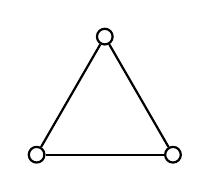
\begin{tikzpicture}
[nodedecorate/.style={shape=circle,inner sep=2pt,draw,thick},%
  linedecorate/.style={-,thick},%
  scale=1]
%% nodes or vertices
\foreach \nodename/\x/\y in {1/0.8660/-0.5, 2/0/1, 3/-0.8660/-0.5} {
  \node (\nodename) at (\x,\y) [nodedecorate] {};
}
%% edges or lines
\path
\foreach \startnode/\endnode in {1/2, 1/3, 2/3} {
  (\startnode) edge[linedecorate] node {} (\endnode)
};
\end{tikzpicture}
}
\qquad
%%
%% graph P_3
\subfigure[$P_3$]{
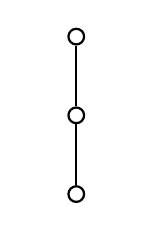
\begin{tikzpicture}
[nodedecorate/.style={shape=circle,inner sep=2pt,draw,thick},%
  linedecorate/.style={-,thick}]
%% nodes or vertices
\foreach \nodename/\x/\y in {1/0/0, 2/0/1, 3/0/2} {
  \node (\nodename) at (\x,\y) [nodedecorate] {};
}
%% stub nodes that should not be visible
\node () at (-0.5,0) [] {};
\node () at (0.5,0) [] {};
%% edges or lines
\path
\foreach \startnode/\endnode in {1/2, 2/3} {
  (\startnode) edge[linedecorate] node {} (\endnode)
};
\end{tikzpicture}
}
\qquad
%%
%% K_3 Cartesian product P_3
\subfigure[$K_3 \square P_3$]{
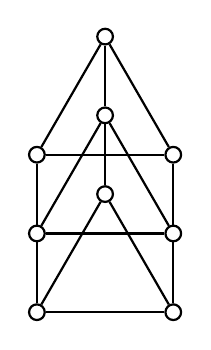
\begin{tikzpicture}
[nodedecorate/.style={shape=circle,inner sep=2pt,draw,thick},%
  linedecorate/.style={-,thick},%
  scale=1]
%% nodes or vertices
\foreach \nodename/\x/\y in {
  %% bottom K_3
  1/0.8660/-0.5, 2/0/1, 3/-0.8660/-0.5,
  %% middle K_3
  4/0.8660/0.5, 5/0/2, 6/-0.8660/0.5,
  %% top K_3
  7/0.8660/1.5, 8/0/3, 9/-0.8660/1.5} {
  \node (\nodename) at (\x,\y) [nodedecorate] {};
}
%% edges or lines
\path
\foreach \startnode/\endnode in {
  %% bottom K_3
  1/2, 1/3, 2/3,
  %% middle K_3
  4/5, 4/6, 5/6,
  %% top K_3
  7/8, 7/9, 8/9,
  %% connecting the K_3 with each other
  1/4, 4/7, 2/5, 5/8, 3/6, 6/9} {
  (\startnode) edge[linedecorate] node {} (\endnode)
};
\end{tikzpicture}
}
